\part{Self-consistent dissipative particle dynamics algorithm}
\frame{\partpage}

\section{欧拉法(Euler)}
\frame{\frametitle{欧拉法}

欧拉法速度和位置的更新如下:

\[
r_i(t+\Delta t) = r_i(t) + v_i(t)\Delta t
\]

\[
v_i(t+\Delta t) = v_i(t) +f_i(t)\Delta t
\]

\[
f_i(t+\Delta t) = f_i\Big(r_i(t+\Delta t), v_i(t+\Delta t)\Big)
\]
}

\frame{\frametitle{欧拉法的缺点}

欧拉法的缺点:
\begin{itemize}
\item 时间步长对体系的平恒特征有影响。比如仿真中理想耗散气体系统的温度。
\[
mk_BT_{eq} = \frac{A_3}{A_1(2-A_1n\Delta t) - A_2\Delta t}
\footnote{Dissipative particle dynamics: The equilibrium for finite time steps. C. A. Marsh and J. M. Yeomans. Europhys. Lett. 37(8), pp. 511-516 (1997)}
\]
其中, $A_1=\frac{\gamma}{md}[w_D]$, $A_2 = \frac{2\gamma^2}{m^2d}[w_D^2]$ $A_3=\frac{\sigma^2}{d}[w_R^2]$
\item 时间步长对径向分布函数有影响。
\item 时间不可逆。
\end{itemize}
}

\section{跳蛙法(leap-frog)}
\frame{\frametitle{跳蛙法(leap-frog)}

跳蛙法(leap-frog)速度和位置的更新如下:

\[
v_i\Big(t+\frac{\Delta t}{2}\Big) = v_i\Big(t-\frac{\Delta t}{2}\Big) + \Delta t\frac{f_i(t)}{m}
\]

\[
r_i(t+\Delta t) = r_i(t) + v_i(t)\Delta t + f_i(t)\frac{(\Delta t)^2}{2m}
\]
}

\frame{\frametitle{跳蛙法的特点}

跳蛙法的特点:
\begin{itemize}
\item 自洽(self-consistently)
\item 时间可逆(time reversible)。
\item 仿真的时间步长不再受算法限制。
\item 计算量更大,需要更多开销。
\end{itemize}
}


\section{算例对比}
\frame{\frametitle{算例对比}

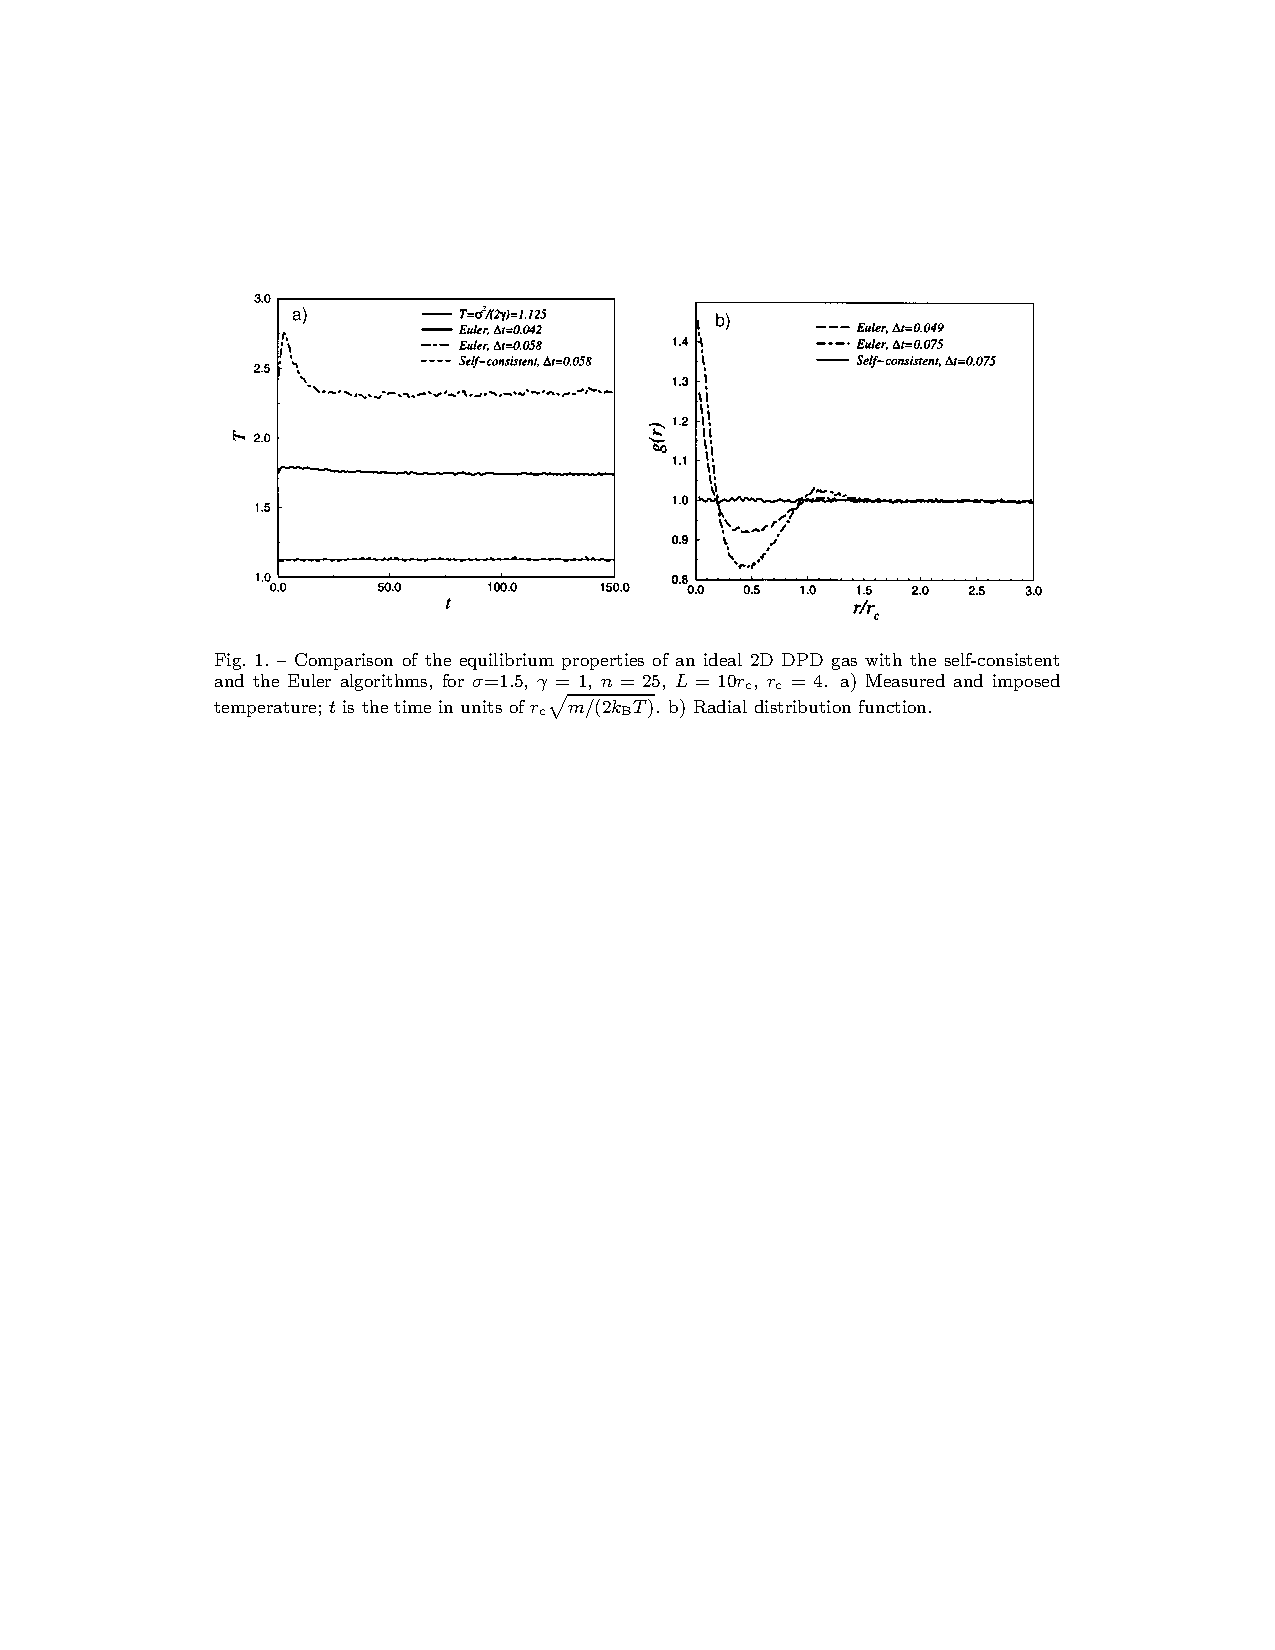
\includegraphics[width=\textwidth]{./figures/Comparison.pdf}
}
